% Systemdokumentation OOP3
% Unterlage für Studenten als Leitfaden für die Erstellung einer SystemDoku
% 17. Oktober 2022
% --- Templates -------------------------------------------------------------
%\includegraphics{}

% Dokumentklasse --------------
\documentclass[12pt,naustrian,a4widepaper]{scrartcl}   
% article style
%   - 11pt Schriftgroesse
%   - new austrian (neue Rechtschreibung)
%   - Papierformat A4
%   - pdf-hyperlinks

% Packages --------
%\RequirePackage{hgblistings}
\usepackage[utf8]{inputenc}  % fuer Umlaute, äöü
\usepackage[T1]{fontenc}
\usepackage{a4wide}
\usepackage{times}      % Times Schriften (zusammen mit fontencoding, s.o.)
\usepackage{babel}
\usepackage{graphicx}	  % für das Einbinden von Grafiken
\usepackage{color}      % für färbigen Text
\usepackage{framed}     % für (Text-) Rahmen
\usepackage{listings}   % für den Sourcecode
\usepackage{fancyhdr}   % für Kopf- und Fusszeilen
\usepackage{pdfpages}	% pdf import fuer angabe

\pagestyle{fancy}       % Kopf- / Fusszeile aktivieren
\lstset{
  language={C++},
  basicstyle=\footnotesize\ttfamily,
  keywordstyle=\color{blue},%\bfseries,
  commentstyle=\color{green},
  frame=single,
  xleftmargin=0pt,
  framexleftmargin=0pt,
  framexrightmargin=0pt,
  linewidth=\dimexpr\textwidth+3cm\relax,
  breaklines=true,
  tabsize=3,
  numbers=left, numberstyle=\tiny, stepnumber=1, numbersep=5pt
}

% Seitenspiegel -------------
\typearea{8}	% Festlegung des Seitenspiegels gem. Koma. 4..groß, 9..klein

% Kopfzeile ---------
\lhead{{\footnotesize{Boris Dobrijevic, Maximilian Ebert}}}   %  (links)
\rhead{{\footnotesize{Seite \thepage}}}      %  (rechts)

% Fusszeile ---------
\lfoot{}  % links
\cfoot{}  % mitte 
\rfoot{}  % rechts

% Absatzformatierung ------------------
\setlength{\parindent}{0cm}   % Einrückung der 1. Zeile jedes Absatzes
\setlength{\parskip}{10pt}    % Abstand zwischen den Absätzen

% Package für Hyperlinks (mit pdf-Optionen) -----------------------------------------
\usepackage[
urlcolor=blue,		% blaue weblinks
linkcolor=black,	% interne Links sind schwarz
colorlinks=true,        % links werden eingefürbt
pdfstartview=FitH,      % PDF-Anzeige: Fensterbreite
pdfborder={0 0 0},      % keine Umrandung um links
pdftitle   ={Systemdokumentation},% Referenzen in der Pdf-Datei
pdfauthor  ={Boris Dobrijevic, Maximilian Ebert},
pdfsubject ={Systemdoku},
pdfcreator ={Der Creator},
pdfproducer={Der Producer},
pdfkeywords={Dokumentation, Systemdokumentation}
]{hyperref}

% =================================================================================================
% =================================================================================================
% Beginn des Dokumentes
\begin{document}
\selectlanguage{naustrian}   % oder "american" für engl. Texte

% Titelblatt ----------
\title {\vspace{1cm}
       \includegraphics[width=8cm]{./Images/FhOOeLogoOkt2009_HSD_Rot_pastell}\\
       \vspace{2cm}
       {\textbf{Systemdokumentation\\Übung 02}}\\
       \vspace{5mm}
       {\small{Version 1.0}}\\
       \vspace{5mm}
}

\author{\small{Boris Dobrijevic, Ebert Maximilian}}
\date  {\small{Hagenberg, \today}}
%\maketitle

\includepdf[pages={1-2}]{Uebung_3_RTO.pdf}
\clearpage

% Inhalts-, Tabellen- und Bildverzeichnis (werden generiert) ----------------------------------------------------------
\tableofcontents

\clearpage
% =================================================================================================
% Kapitel 1 ---------------------
\section{Aufgabe A: Erweiterung prioritätsbasiertes Scheduling}

Durch das Einführen von Prioritäten wird der Round-Robin-Scheduler zu einem prioritätsbasierten, präemptiven Scheduler mit Round-Robin-Verfahren erweitert.
Jedem Task wird eine Priorität zugewiesen.
Ein höherer numerischer Wert entspricht einer höheren Priorität.
Ein Task mit höherer Priorität verdrängt sofort einen laufenden Task mit niedrigerer Priorität (z.B. wenn der höher prioritäre Task durch ein Event oder Timer bereit ("Ready") wird).
Tasks mit identischer Priorität teilen sich die CPU-Zeit basierend auf Time Slices.
Wenn die Zeitscheibe eines Tasks abläuft und ein anderer Task gleicher Priorität wartet, erfolgt ein Kontextwechsel.

\subsection{Implementierung der Datenstrukturen}
Der Task Control Block (TCB) in \texttt{APOS.h} wurde um einen pNextRdy pointer erweitert, welcher genutzt wird, um eine Ready-Queue zu verwalten.

\begin{lstlisting}[language=C, caption={Erweiterter TCB in APOS.h}]
struct APOS_TCB_STRUCT {
    ...
    struct APOS_TCB_STRUCT* pNextRdy;
};
\end{lstlisting}

Die Ready-Queue wird als einfach verkettete Liste organisiert, die stets nach Priorität sortiert ist.
Der Zeiger pHead zeigt immer auf den Task mit der höchsten Priorität, der aktuell bereit ist.

\subsection{Scheduler Logik}
Die Funktion \texttt{APOS\_INSERT\_QUEUE} in APOS.c sorgt dafür, dass Tasks sortiert eingefügt werden.
Tasks mit höherer Priorität werden vor Tasks mit niedrigerer Priorität platziert. Bei gleicher Priorität wird der neue Task hinter den bestehenden Tasks dieser Prioritätsstufe eingereiht (FIFO-Prinzip innerhalb der Priorität).
Somit erfolgt bei gleichen Prioritäten immer noch das Round-Robin-Prinzip.
\\
\\
Der Scheduler wählt im Normalfall einfach den ersten Task der Liste (\texttt{pHead}) aus, da die Liste sortiert ist.
Die Round-Robin-Logik greift, wenn die Zeitscheibe abgelaufen ist:

\subsection{Preemption im SysTick}
Der \texttt{SysTick\_Handler} in \texttt{systick.c} prüft jede Millisekunde, ob ein Kontextwechsel notwendig ist. 
Dies geschieht in zwei Fällen:
Ein Task mit höherer Priorität ist bereit geworden (\texttt{pHead->Priority > pCurrentTask->Priority}) oder die Zeitscheibe des laufenden Tasks ist abgelaufen (\texttt{TimeLeft == 0}).
Die Preemption wird durchgeführt, falls ein Task im Start der Liste (am pHead) eine höhere Prio als der currentTask hat.

\subsection{Prüfen der Preemption und Prioritäten}
Um die Priority zu Prüfen werden die drei in der Angabe geforderten Prioritäten für den Counter eingetragen.

\clearpage
\subsubsection{Priority 1}
Hier ist zu sehen, dass der Counter Task nie ausgeführt wird.
Dies geschieht, weil der Task durch seine geringe Priorität nie in der Ready-Queue nach oben wandert.
Somit wird dieser Task immer durch einen anderen Task verhindert.\\
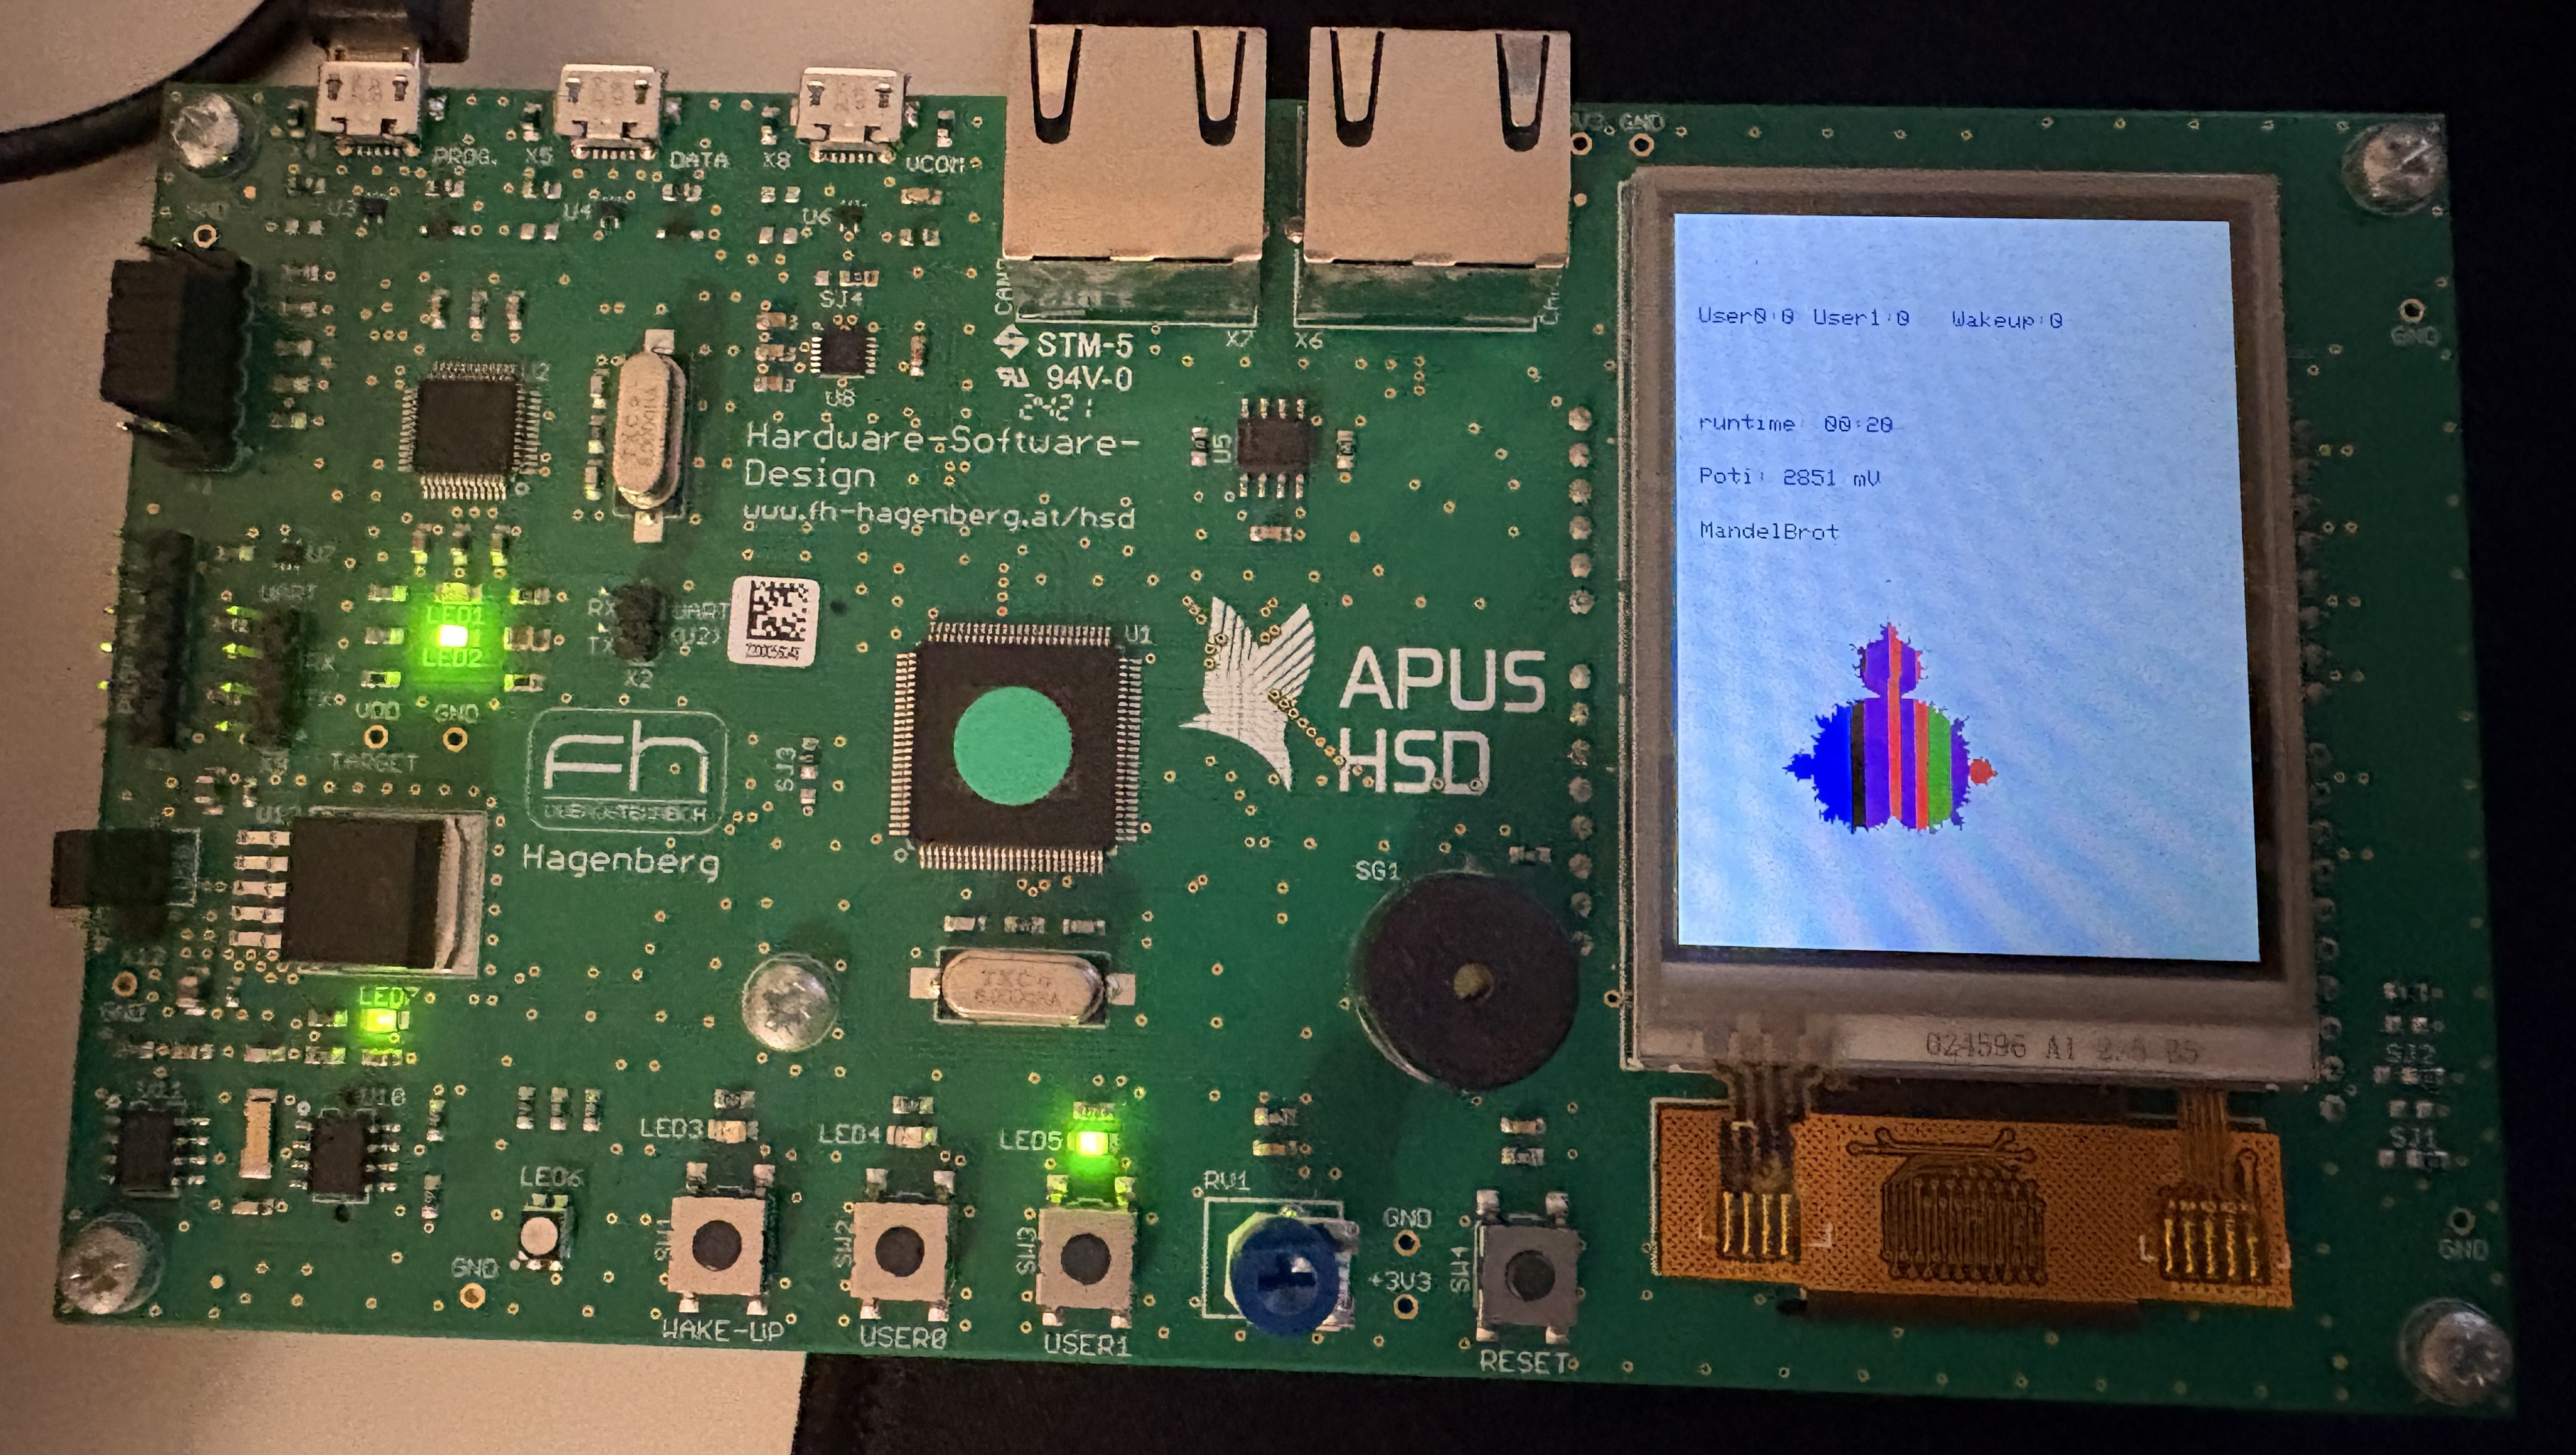
\includegraphics[width=.9\textwidth]{Images/IMG_6075.jpg}\\
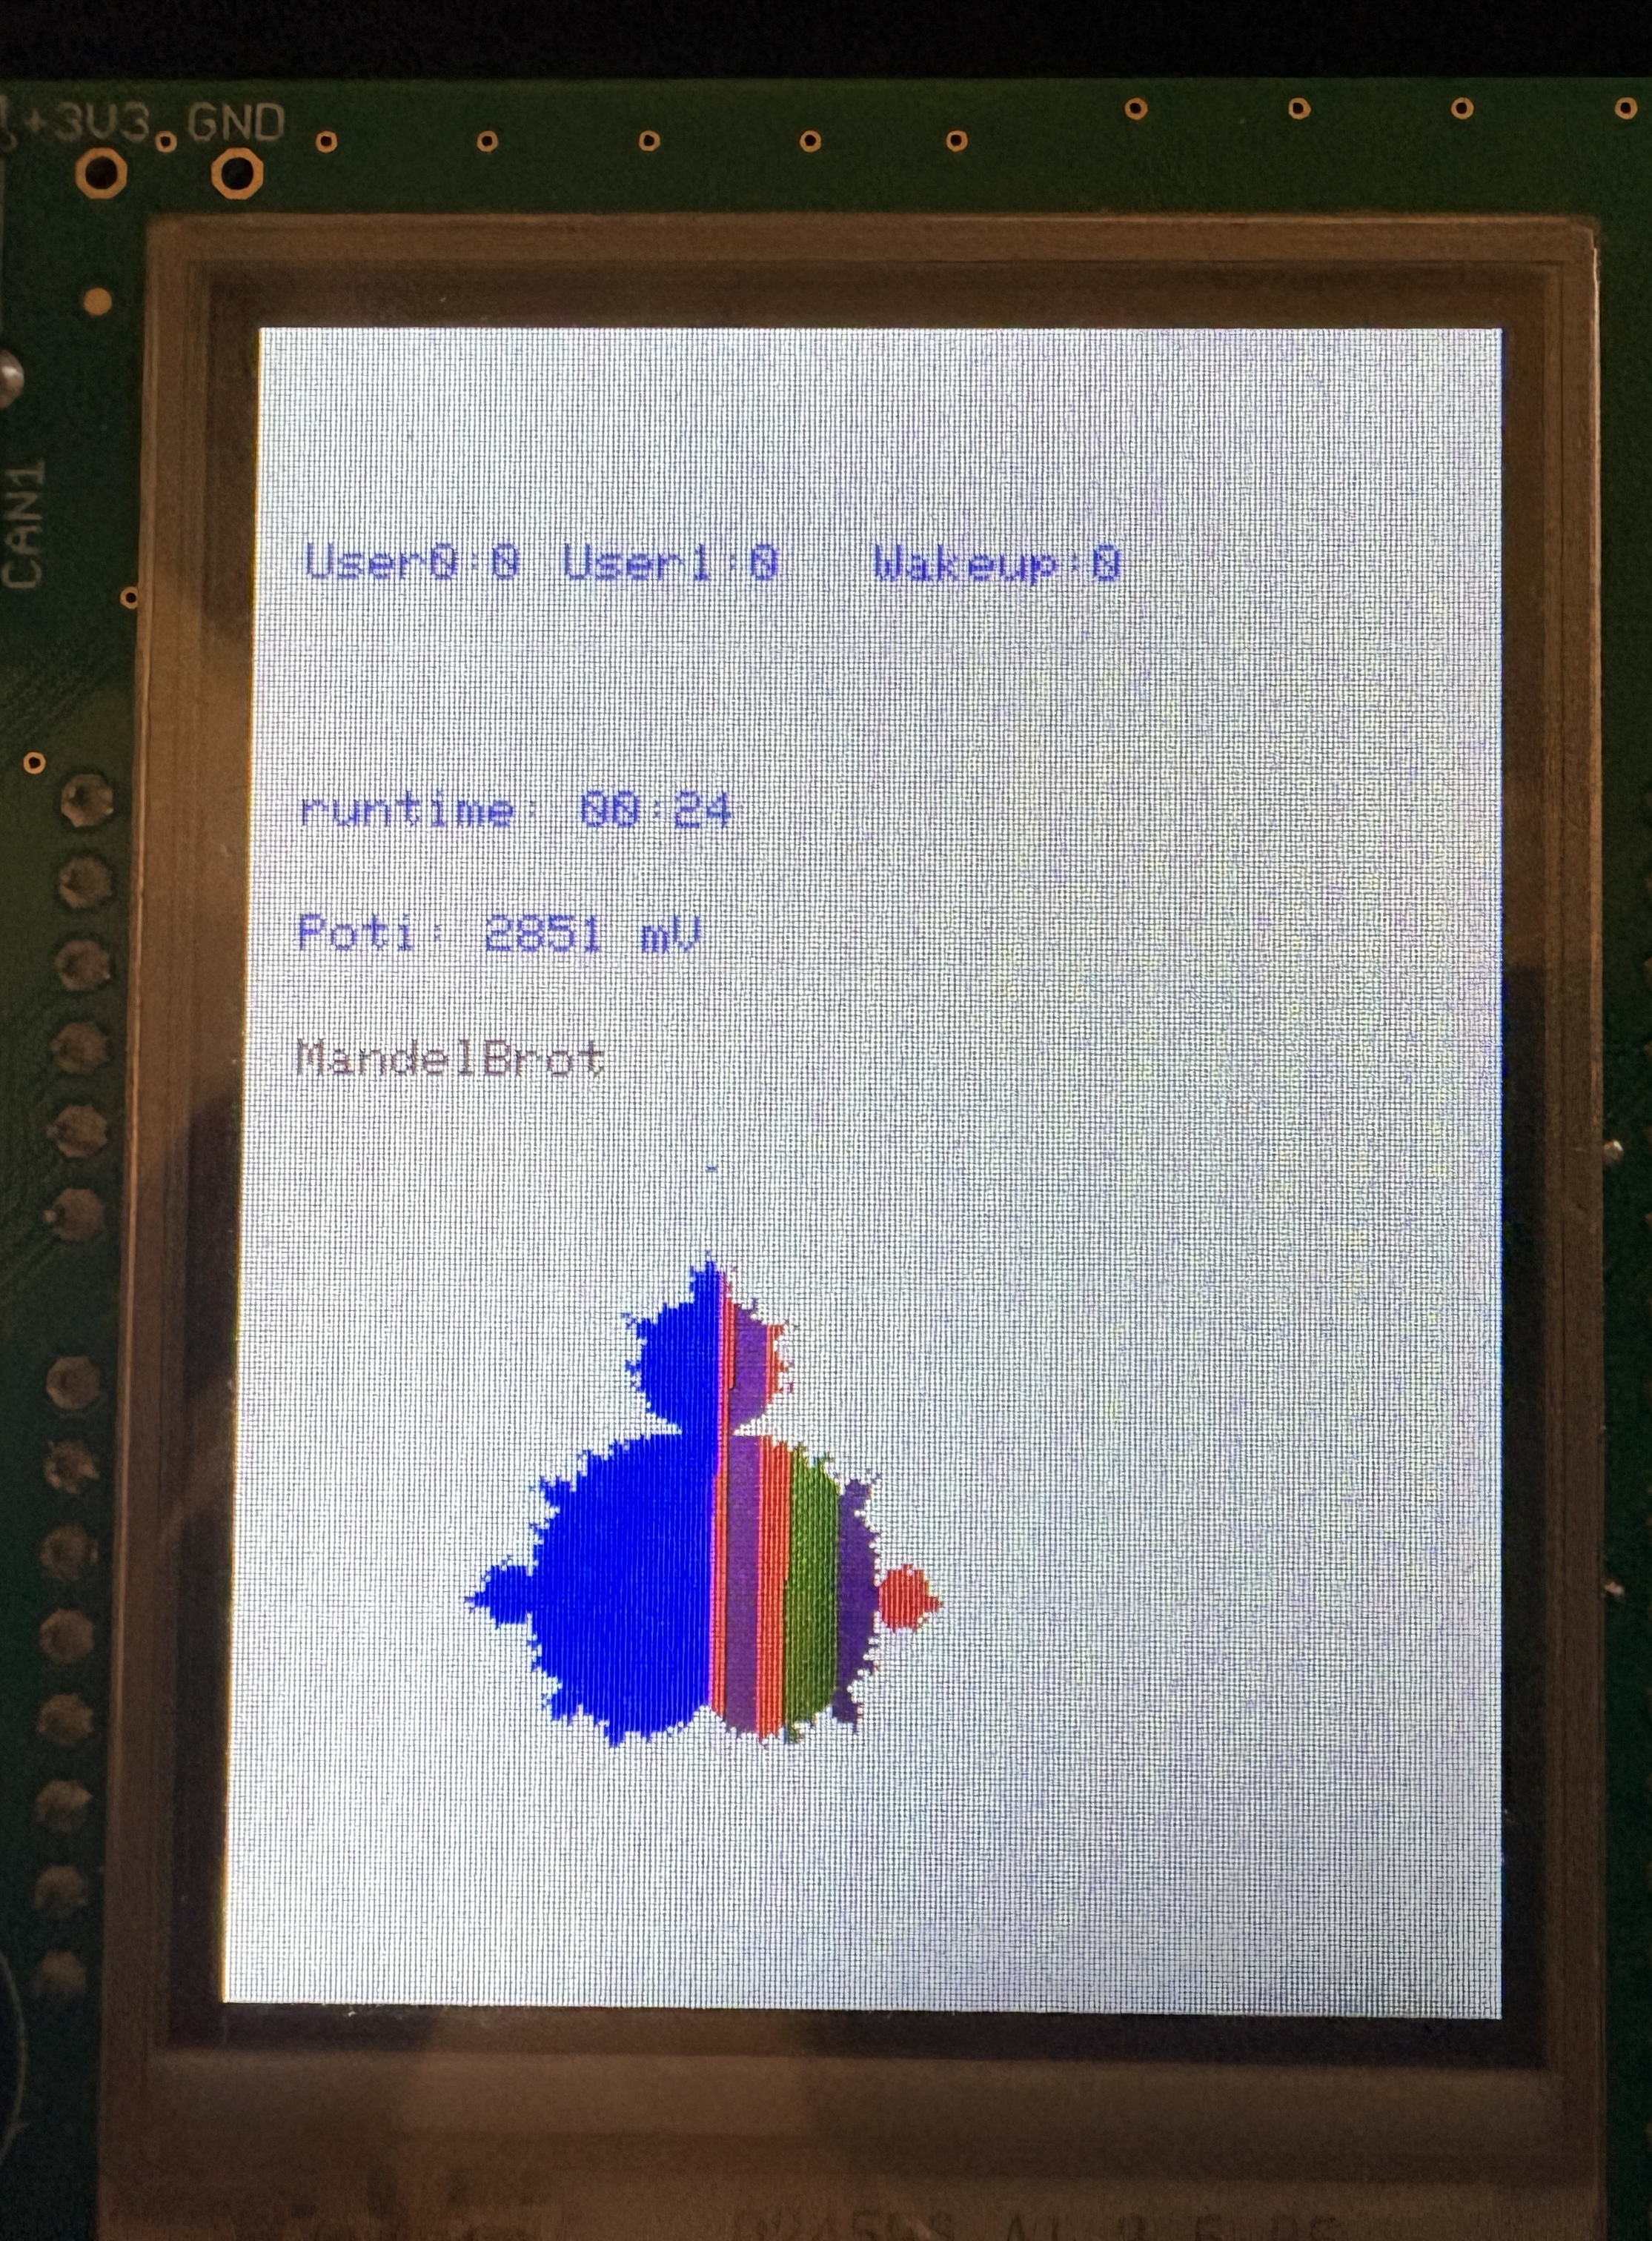
\includegraphics[width=.5\textwidth]{Images/IMG_6076.jpg}\\

\subsubsection{Priority 100}
Bei Priority 100 haben alle Tasks, bis auf den NOP-Task, die selbe Priorität.
Somit wird ein Task, nachdem er durchläuft, einfach wieder hinten in der Ready-Queue eingereiht.
Hierbei ist kein Unterschied zwischen der jetztigen und der bisherigen Round-Robin-Implementierung zu erkennen.\\
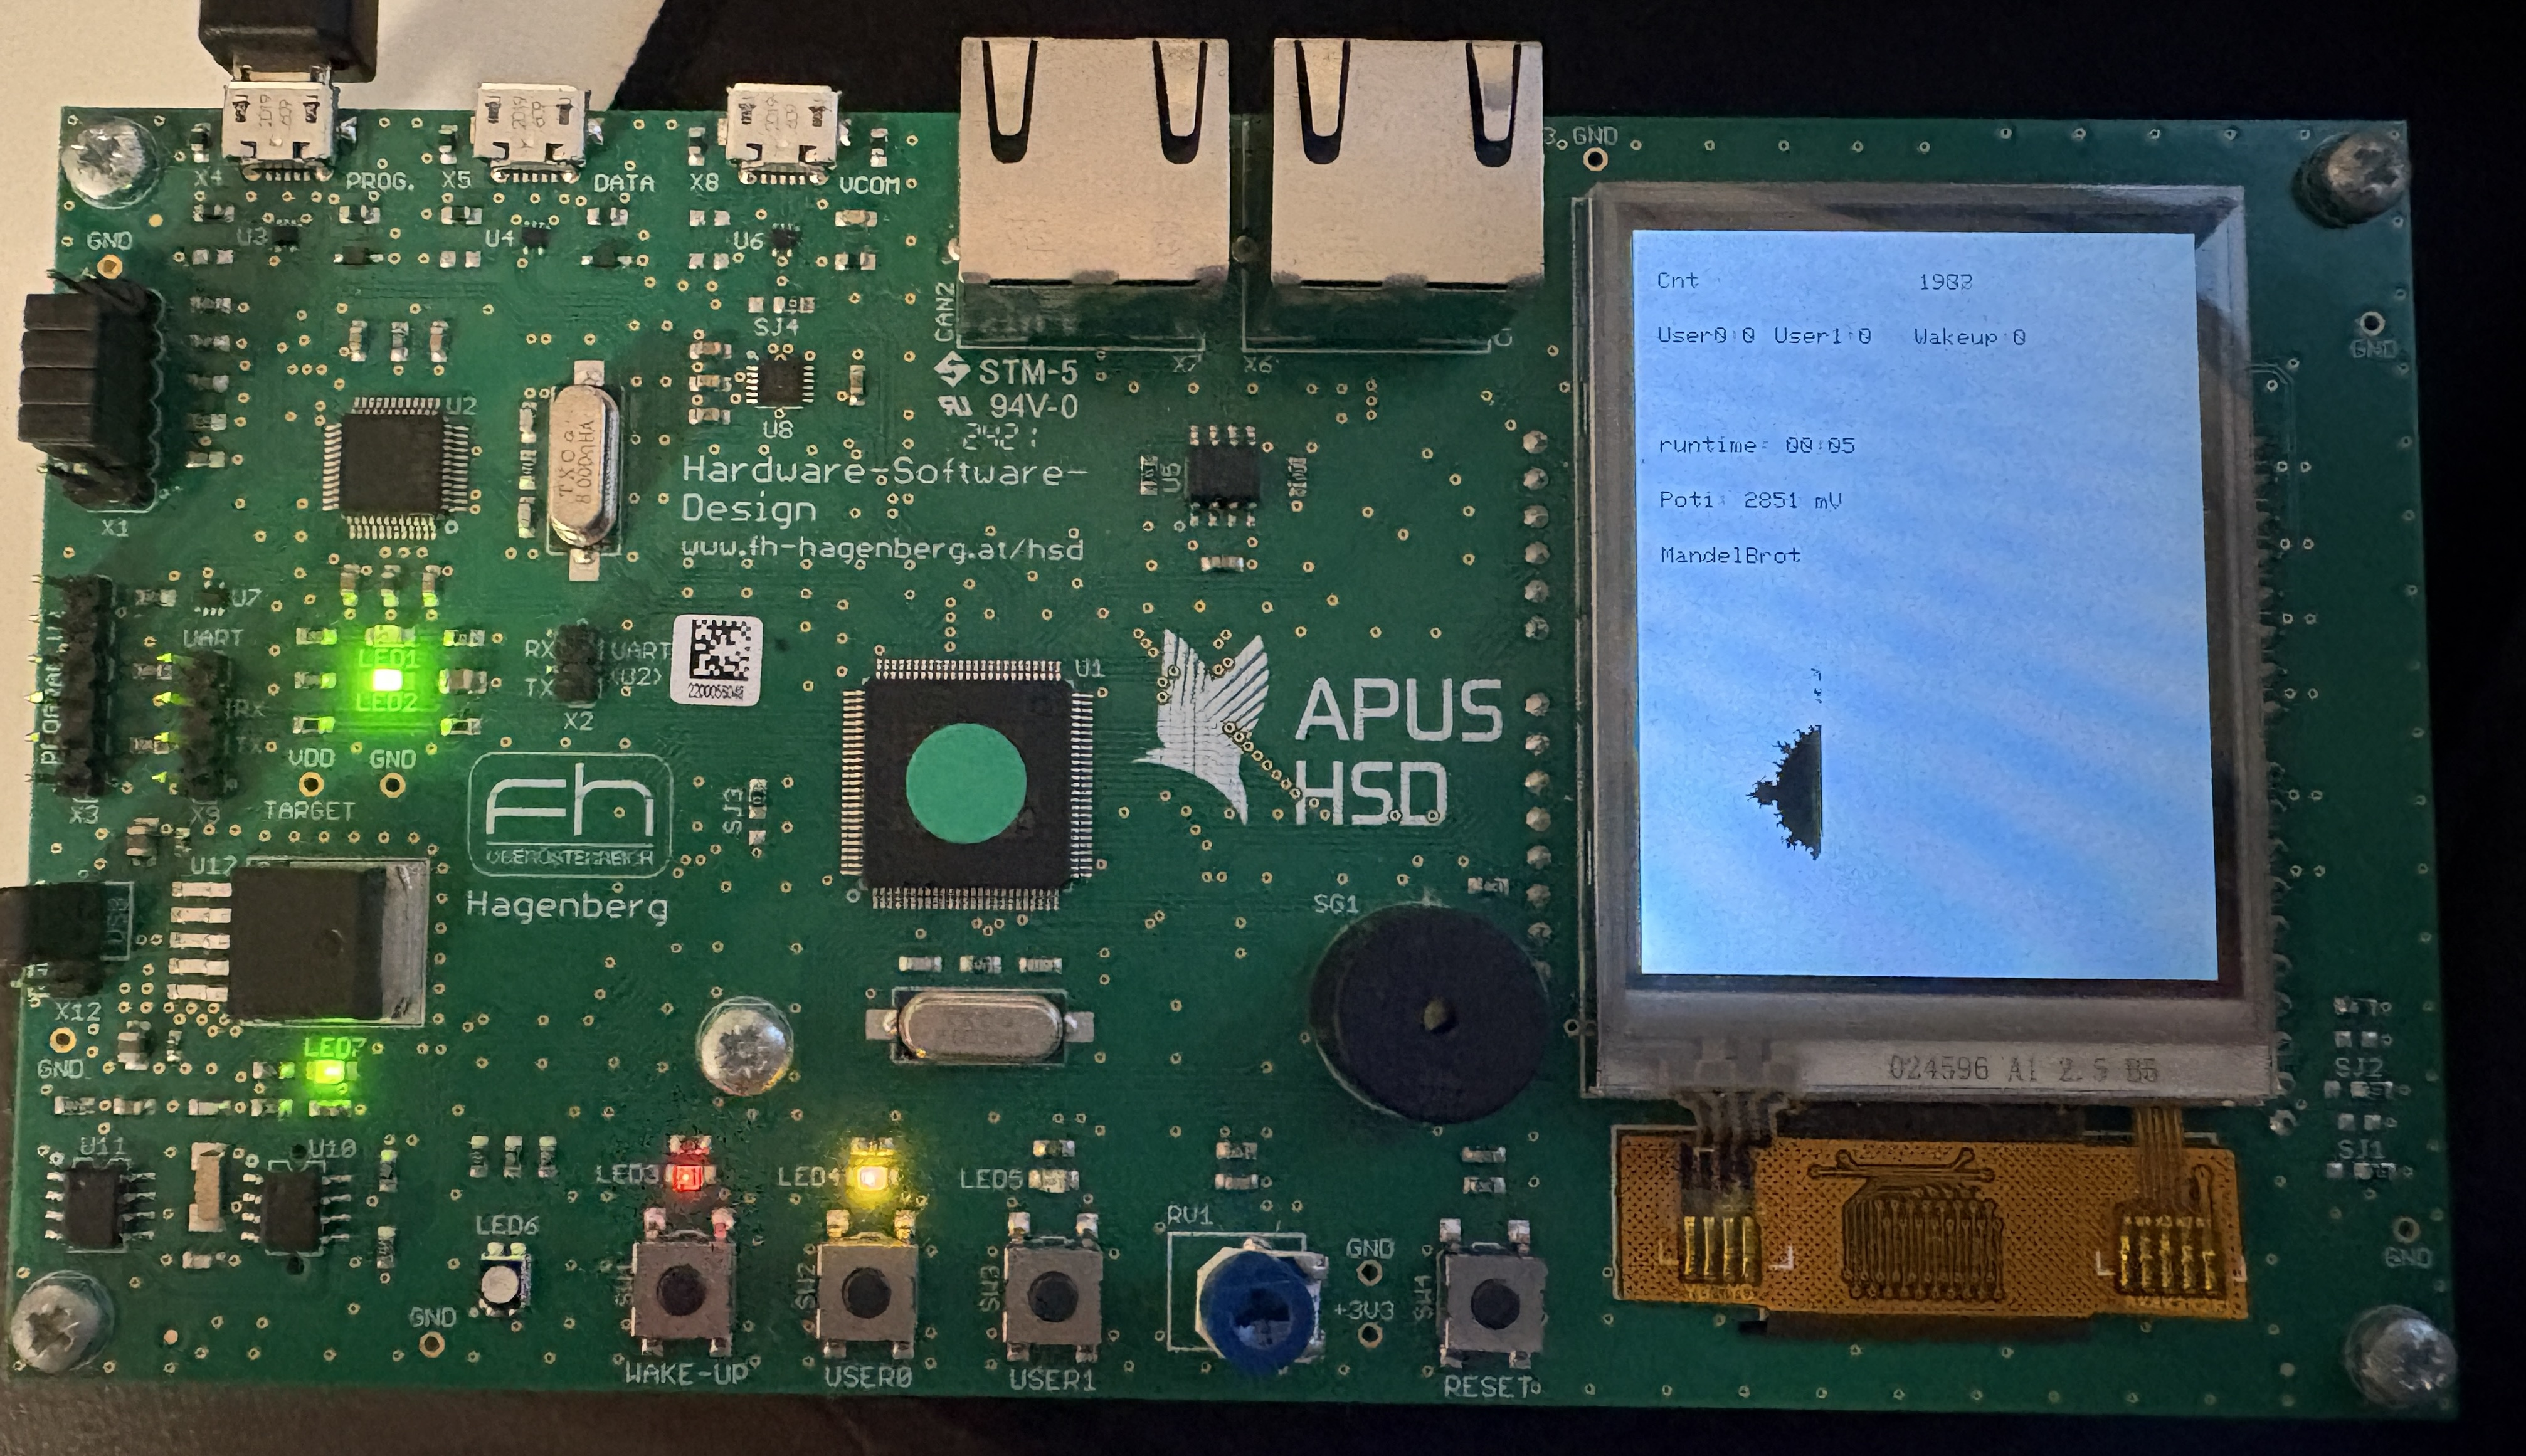
\includegraphics[width=.9\textwidth]{Images/IMG_6077.jpg}\\
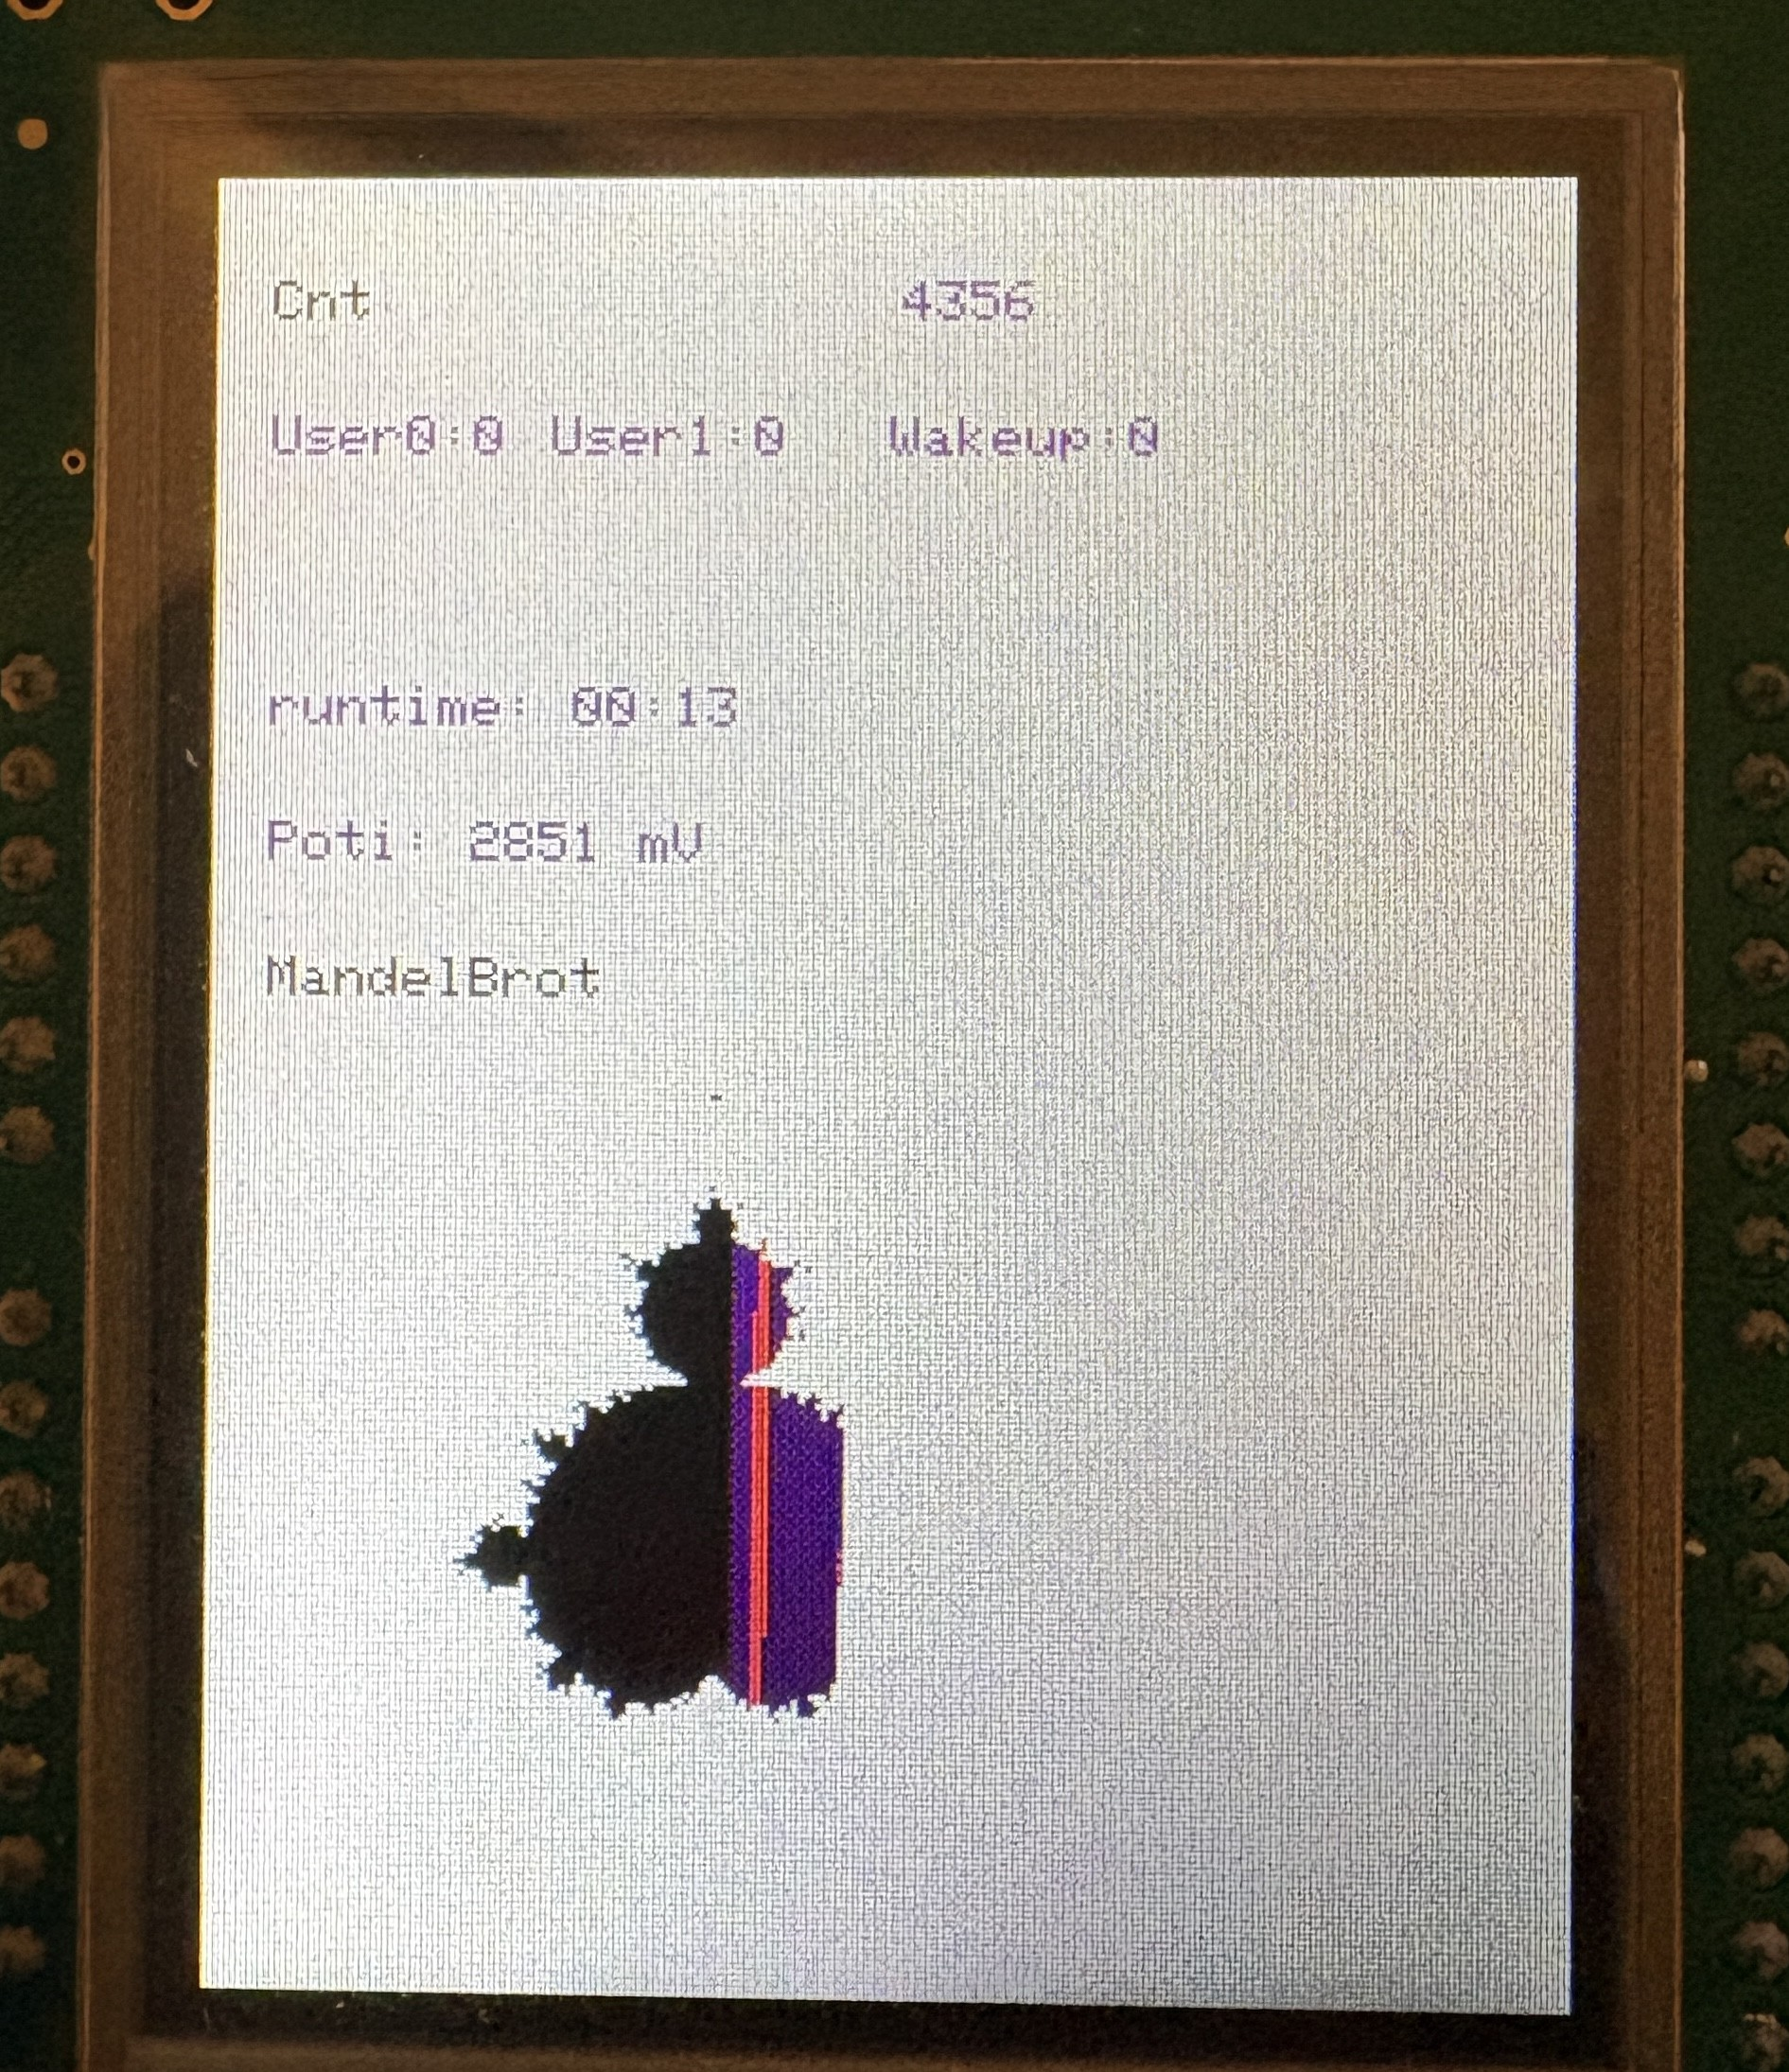
\includegraphics[width=.5\textwidth]{Images/IMG_6078.jpg}\\

\subsubsection{Priority 200}
Das Verhalten bei Counter Prio 200 ist das Gegenteil von Prio 1, insbesondere weil der Counter-Task keinen Delay besitzt, wodurch er die CPU-Zeit freiwillig freigibt.
Dadruch wird der Task nach Ablauf der Zeit sofort wieder an der Spitzte der Ready-Queue eingereiht und läuft sofort wieder weiter.
Somit kommt kein weiterer Task dran und nur der Counter-Task kann laufen.
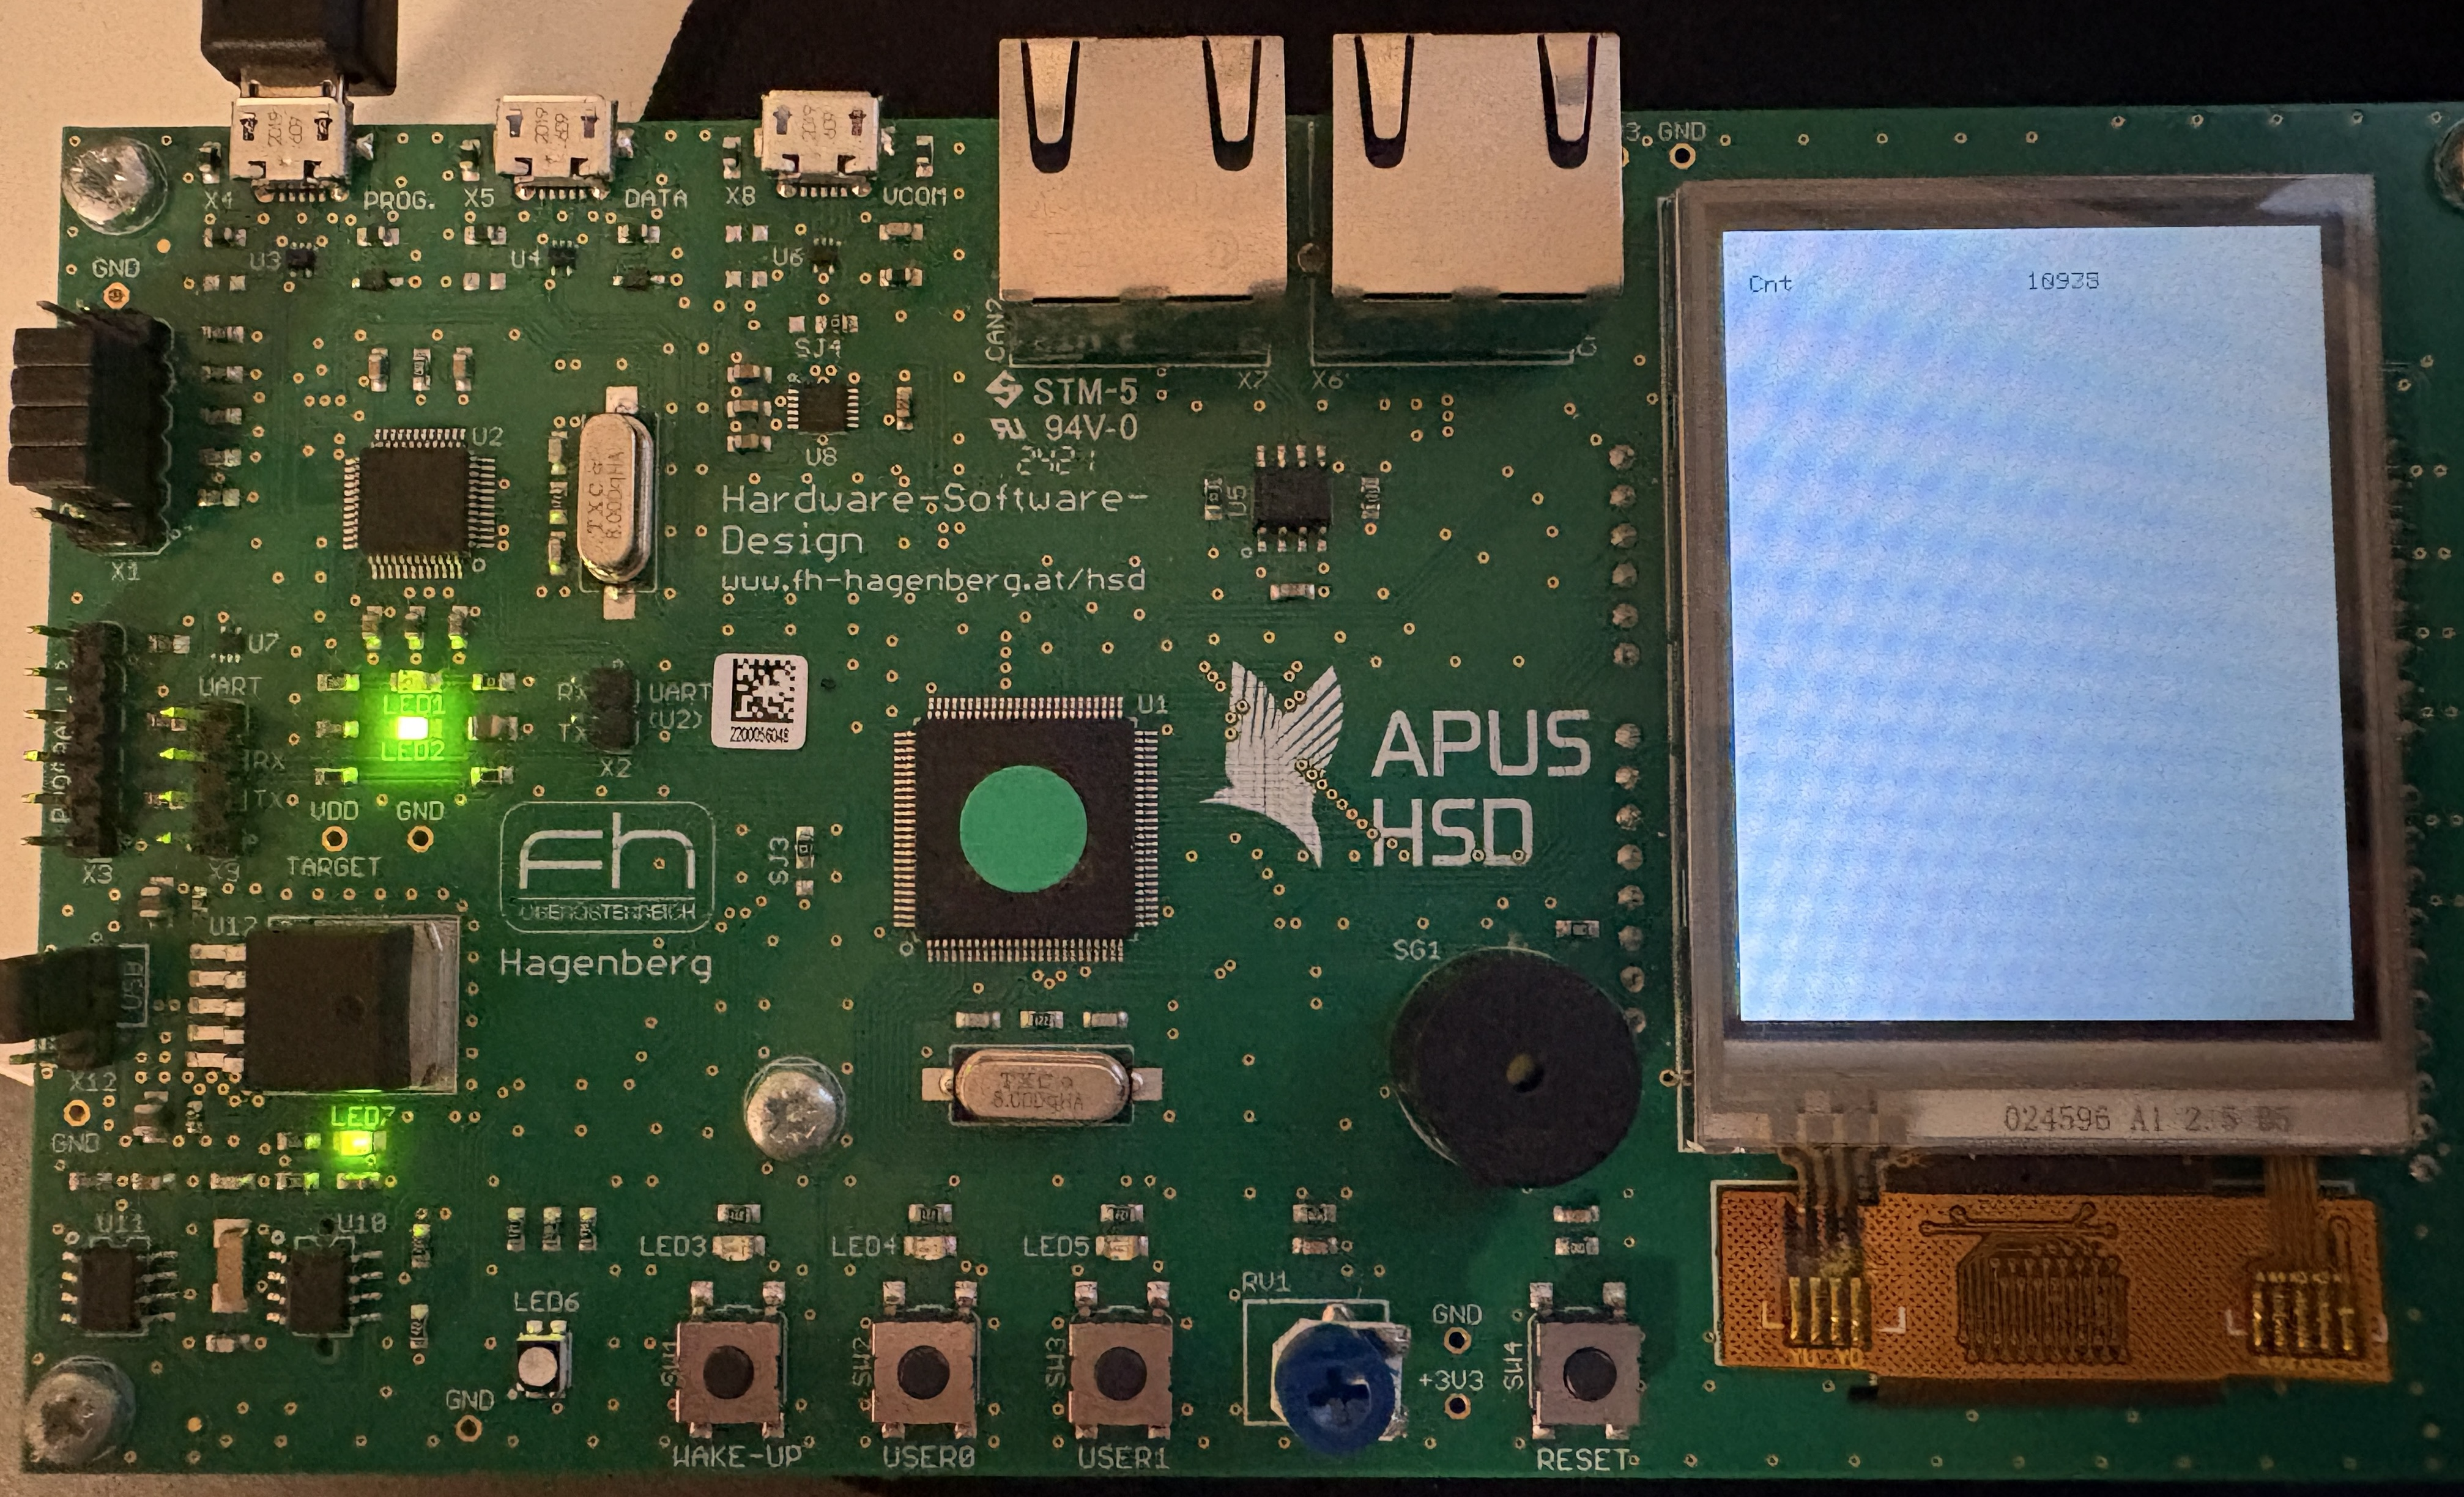
\includegraphics[width=.9\textwidth]{Images/IMG_6079.jpg}\\
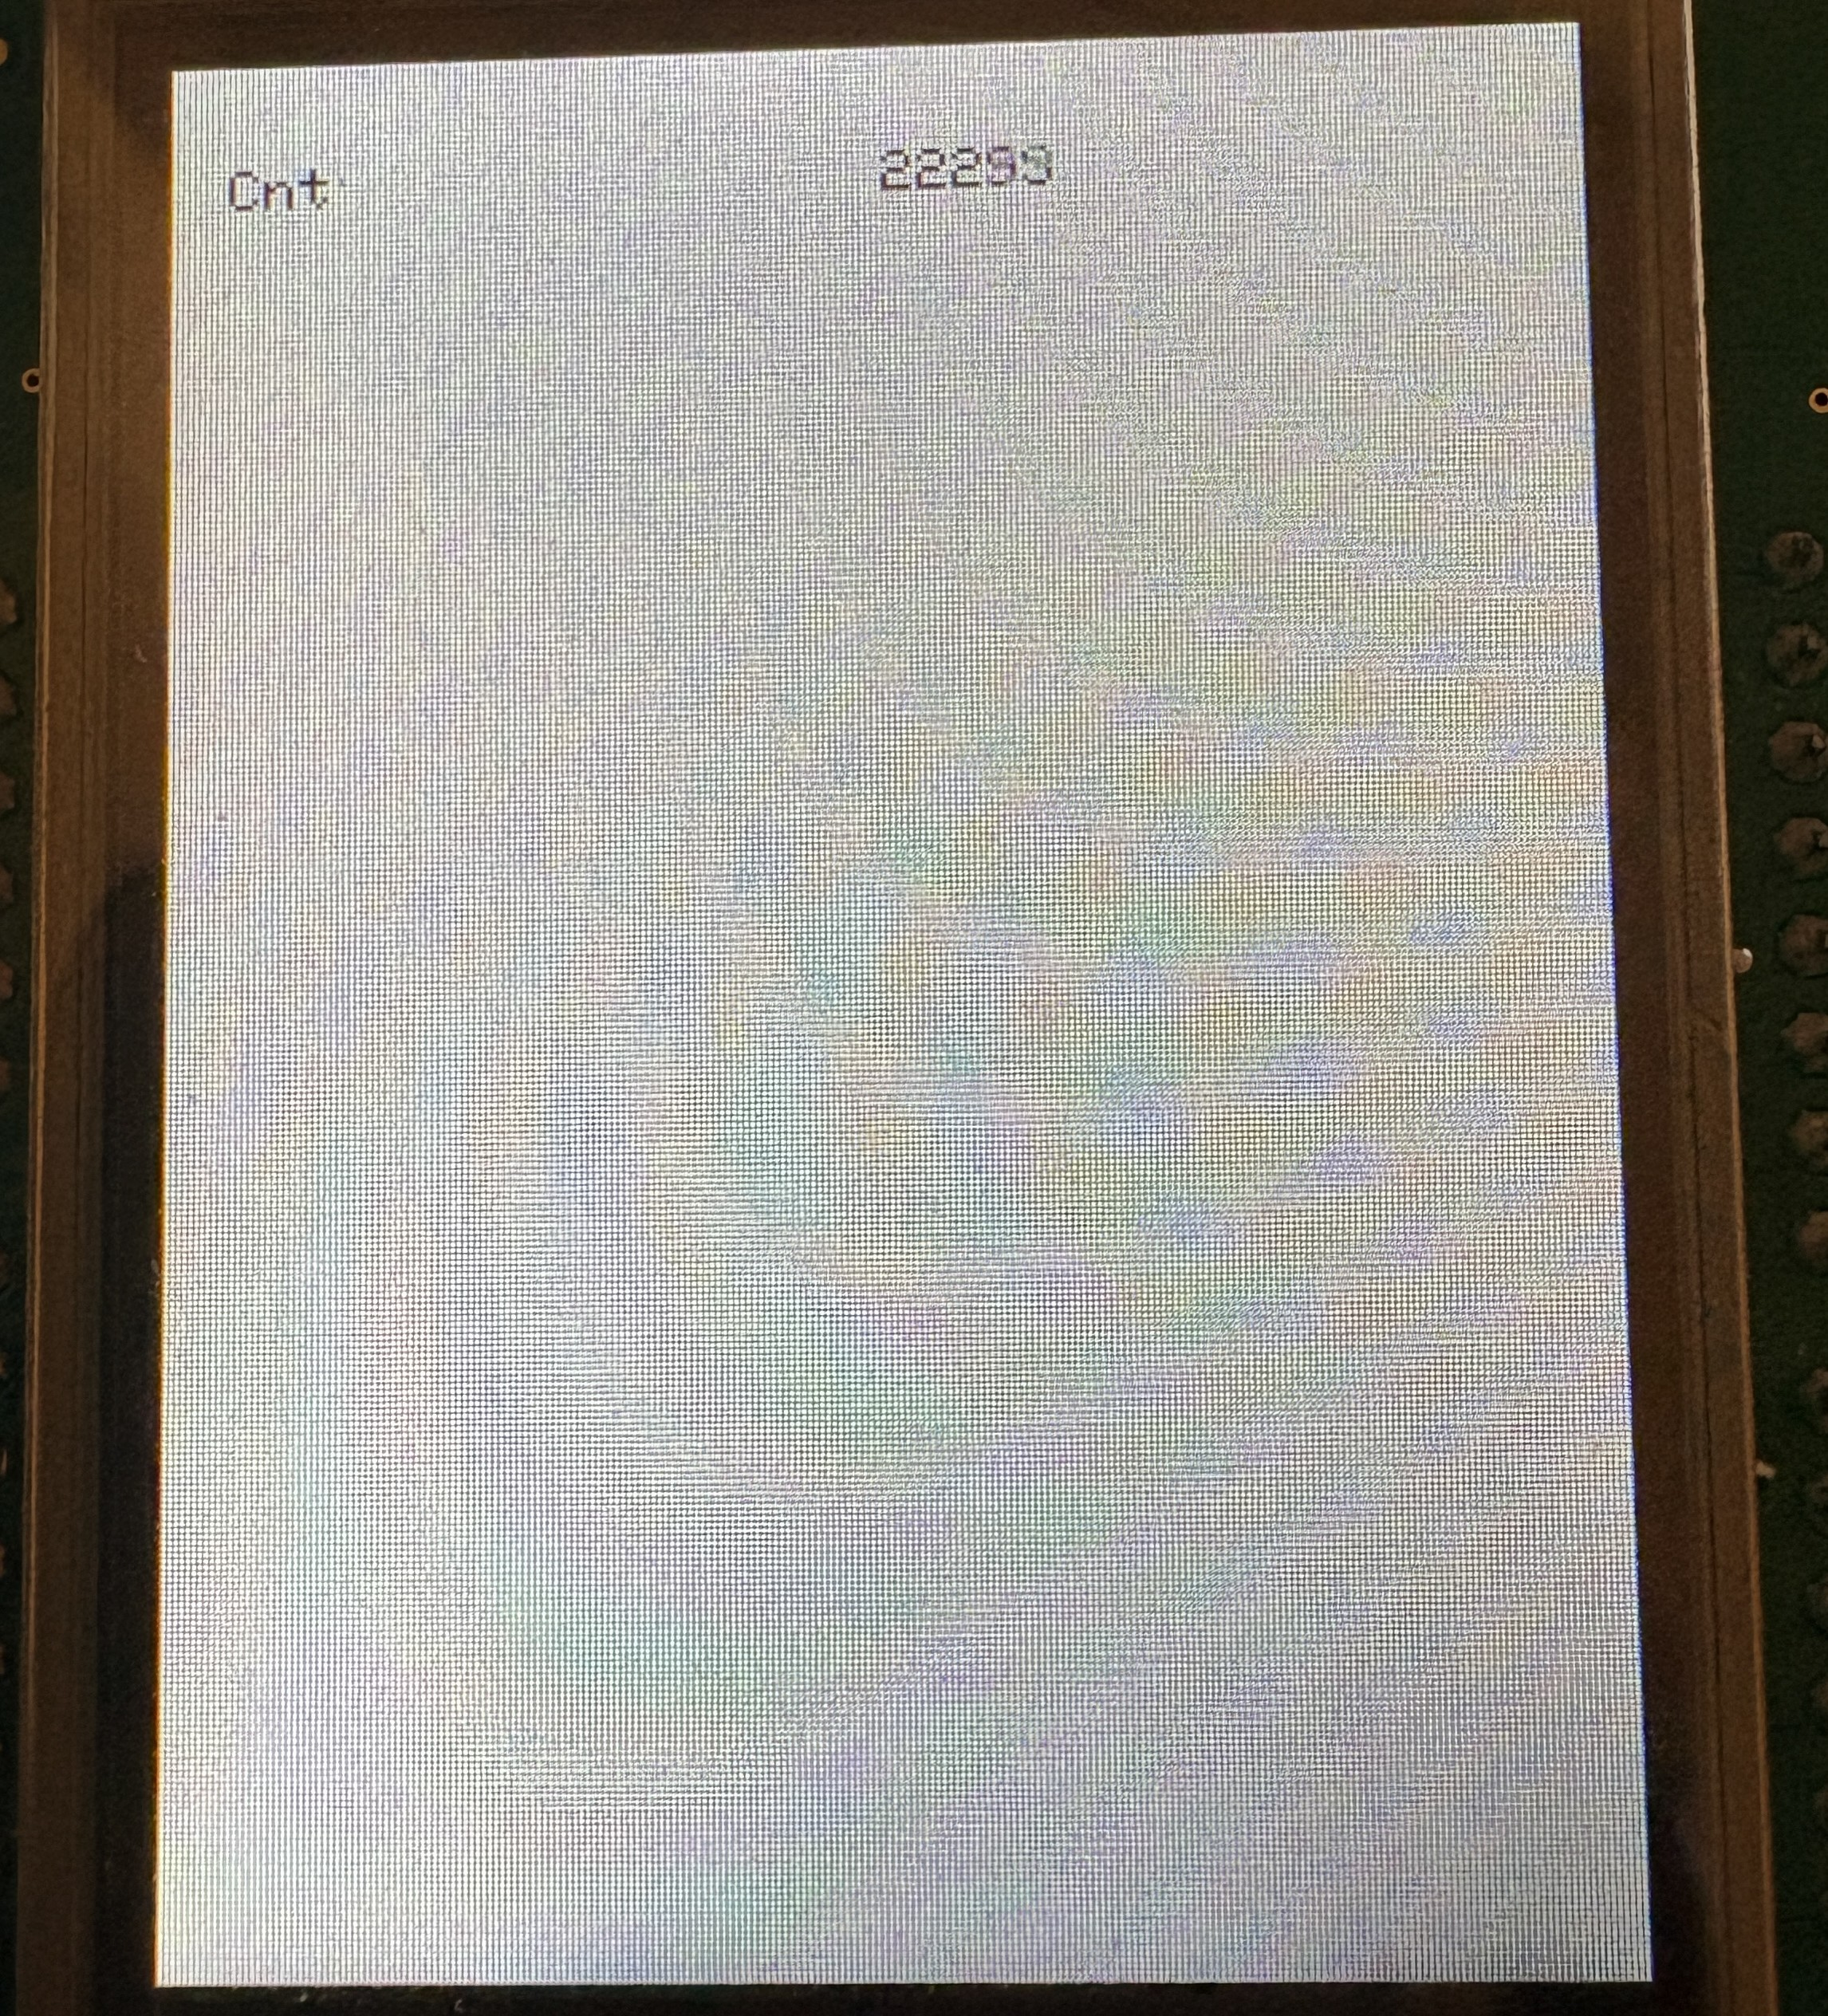
\includegraphics[width=.5\textwidth]{Images/IMG_6080.jpg}\\

\subsection{Vor- und Nachteile}
\textbf{Vorteile}\\
Diese Implementierung mittels Ready-Queue und Preemption bietet einige Vorteile.
Der größte Vorteil ist die Reaktionszeit für hochpriorisierte Tasks.
Tritt ein Task mit hoher Priorität in die Ready-Queue ein, so wird ein laufender Task mit niedrigerer Priorität sofort unterbrochen. 
Dies minimiert die Latenzzeit für wichtige Systemkomponenten.
\\
\\
Da die Ready-Queue als sortierte verkettete Liste implementiert ist, ist die Entscheidung, welcher Task als nächstes läuft, sehr effizient.
Der Scheduler muss nicht durch alle Tasks iterieren, sondern wählt immer das erste Element (pHead).
Dies reduziert den Overhead im SysTick\_Handler und beim Kontextwechsel.
\\
\\
Durch den Round-Robin-Algorithmus wird verhindert, dass sich Tasks mit gleicher Wichtigkeit gegenseitig blockieren.
Ein rechenintensiver Task (z.B. Mandelbrot-Berechnung) kann so gleichzeitig mit einem UI-Task laufen, ohne dass die UI einfriert.
Das System erlaubt dadurch eine Mischung aus Hintergrundaufgaben mit niedriger Prio und wichtigen, kurzweiligen Vordergrundaufgaben mit hoher Prio.
\\
\\
\textbf{Nachteile}\\
Ein Problem bei diesem Verfahren ist, dass Tasks mit niedriger Priorität selten bis gar nicht zur Ausführung kommen, wenn Tasks mit höherer Priorität dauerhaft Ready sind und Großteile der CPU-Zeit beanspruchen.
In der aktuellen Implementierung läuft der Counter Task bei einer Prio von 1 niemals, solange der Mandelbrot-Task mit Prio 100 rechnet.
Hierbei ist dieser Task besonders problematisch, da er sich selbstständig nie in den Delay versetzt.
\\
\\
Während die Auswahl des nächsten Tasks sehr schnell ist, mit einer Laufzeitkomplexität von ($O(1)$), ist das Einfügen eines Tasks in die Ready-Queue linear abhängig von der Anzahl der bereiten Tasks ($O(N)$).
Bei sehr vielen Tasks könnte dies die Zeit, die innerhalb critical sections Sektionen oder ISRs verbracht wird, verlängern.

% =================================================================================================
% Kapitel 2
\section{Aufgabe B: Einbau eines Stack-Checkers}

Der Stackguard wird bei jedem Taskswitch geprüft.
Als Stackguard wird ein 8-Byte-String verwendet, der bei der Initialisierung an das Ende jedes Taskstacks geschrieben wird:
\begin{verbatim} #define APOS_STACK_GUARD "STACKEND" \end{verbatim}

\textbf{Stackguard Messung:}\\
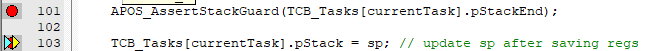
\includegraphics[width=1\textwidth]{Images/StackguardMessung.png}\\
\textbf{Vorher:}\\
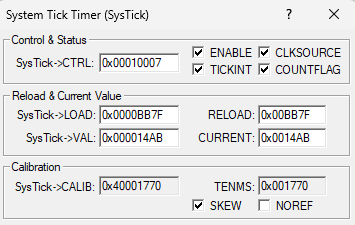
\includegraphics[width=1\textwidth]{Images/StackguardVorher.png}\\
\textbf{Nachher:}\\
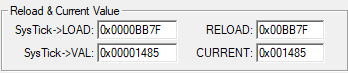
\includegraphics[width=1\textwidth]{Images/StackguardNachher.png}\\

\textbf{Stackguard runtime Berechnung}
0x14Ab - 0x1485 = 0x26
Dies entspricht 38 Cycles in Dezimal.
Mit CoreClock 48MHz ergibt sich ein Laufzeit-Overhead durch den Stackguardcheck von 38*1/48MHz = 792ns.

Die gemessene Laufzeit gilt ausschließlich für den Normalfall mit intaktem Stack-Guard.
Im Fehlerfall entsteht ein zusätzlicher Laufzeit-Overhead, der jedoch keine praktische Relevanz besitzt, da die Applikation in diesem Szenario in einen Fehlerzustand übergeht.


\textbf{Fehlerfall}\\
Händische Änderung des Stackguards:\\
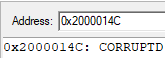
\includegraphics[width=1\textwidth]{Images/StackguardCorrupted.png}\\\\
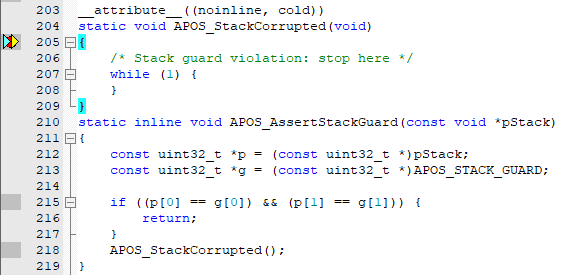
\includegraphics[width=0.9\textwidth]{Images/StackguardFunction.png}\\

Der Stack-Guard funktioniert wie vorgesehen. Bei einer Veränderung des Stack-Guards wird die Funktion APOS\_StackCorrupted() aufgerufen, woraufhin die Applikation in einer Endlosschleife verbleibt.



\section{Aufgabe C: Task-Event-Handling}

\subsection{TaskLed und TaskKey}

Task Led wird nach jedem Tastendruck in WaitingEvent state versetzt:
\begin{figure}[h!]
	\centering
	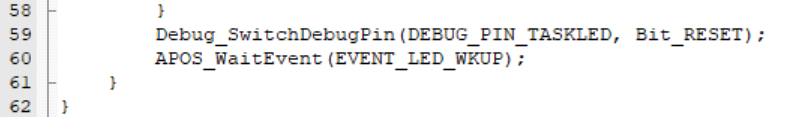
\includegraphics[width=0.7\linewidth]{Images/TaskLed}
	\caption{Task Led APOS Event}
	\label{fig:taskled}
\end{figure}

Bei Tastendruck (beliebige Taste) wird Event an TaskLed geschickt. Gedrückthalten der Taste lässt das Lauflicht in 100ms Takt laufen:

\begin{figure}[h!]
	\centering
	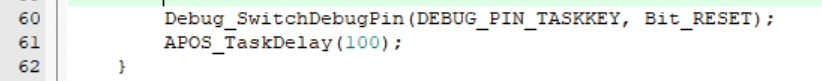
\includegraphics[width=0.7\linewidth]{Images/TaskKey}
	\caption{TaskKey: Signalisiert Event für TaskLed}
	\label{fig:taskkey}
\end{figure}

\subsection{Erweiterung APOS Events}

Der TCB wird um die 32-bit Bitmasken events und waitForEvents erweitert.
Mit events werden durch APOS\_SignalEvent signalisierte Tasks registriert.
Mit waitForEvents wird mit der Funktion APOS\_WaitEvent(..) registriert, durch welche Events der Task aufgeweckt werden kann.

Wird ein Signal registriert wird es in der events maske gesetzt und es wird geprüft, ob der Task auf ein Event wartet (state APOS\_TASK\_WAITING\_EVENT) und ob das signalisierte event in der gespeicherten WaitForEvents maske enthalten ist.
 
In diesem Fall wird der Task auf Status ready gesetzt und in die Ready queue aufgenommen. Falls der aufgeweckte Task an Spitze der ready queue ist und höhere Priorität als der derzeitige Task hat, wird ebenfalls ein TaskSwitch ausgeführt.
 
In der APOS\_WaitEvent Funktion wird die bitmaske zum aufwecken des Tasks übergeben. Der Task wird in den State APOS\_TASK\_WAITING\_EVENT versetzt und erst wieder aufgeweckt, wenn anderer Task das entsprechende Event auslöst.
Nach aufwecken wird die eventmaske zurückgegeben und gelöscht.

Mit der APOS\_ClearEvents Funktion wird die Eventmaske des Tasks gelöscht. Die gelöschten Events werden als Rückgabewert übergeben.

Zur Vermeidung von Raceconditions sind diese Funktionen mit Criticalsections versehen.  

\subsection{Vorteile / Nachteile der Implementierung}

Vorteile der Implementierung:
\begin{itemize}
	\item Nutzung von bitmasken einfach zu implementieren
	\item Jeder Task besitzt Möglichkeit auf bis zu 32 Events zu warten, mit wenig Overhead (2x 32bit maske) pro Task.
	\item Event kann durch beliebige Tasks ausgelöst werden. TaskLed ist von Auslöser des Events entkoppelt.
\end{itemize}

Nachteile der Implementierung:
\begin{itemize}
	\item Keine Queue für Events: werden bis zum Aufwecken des Tasks mehrere Events ausgelöst, wird dies nur einmalig registriert.
	\item Gefahr von Deadlocks: Die derzeitige Implementierung verhindert nicht, dass Deadlocks auftreten können falls Tasks auf ein Event des jeweils anderen Tasks warten.
	\item Scheduler Priorität entscheidend: Ist die Priorität des aufgeweckten Tasks niedriger als die des ausführenden Tasks, wird der Task trotz Event nicht sofort ausgeführt (kann auch als Vorteil interpretiert werden).
\end{itemize}

% #################################################################################################
%      Quellcode
% #################################################################################################
\clearpage
\section{Quellcode}
 \subsection{main.c}
 \lstinputlisting{../../Uebung3/src/main.c}
 \subsection{APOS.h}
 \lstinputlisting{../../Uebung3/src/APOS.h}
 \subsection{APOS.c}
 \lstinputlisting{../../Uebung3/src/APOS.c}
 \subsection{TaskKey.h}
 \lstinputlisting{../../Uebung3/src/Tasks/TaskKey.h}
 \subsection{TaskKey.c}
 \lstinputlisting{../../Uebung3/src/Tasks/TaskKey.c}
 \subsection{TaskLed.h}
 \lstinputlisting{../../Uebung3/src/Tasks/TaskLed.h}
 \subsection{TaskLed.c}
 \lstinputlisting{../../Uebung3/src/Tasks/TaskLed.c}


\end{document}
